\chapter{Background}

In this chapter, an introduction to the GPU architecture, CUDA programming environment, and network IDS is presented.

\section{Network Intrusion Detection System (NIDS)}
Network IDSs collect the packets that pass through the network and check if the packets are legitimate. When an IDS identifies any suspicious activity, it either logs the activity or alerts the network administrator about the activity. An example of NIDS is Snort \cite{bib11}. Snort uses thousands of signatures to detect malicious activities in the packets that are flowing across the network. There are two types of NIDS, signature-based NIDS and machine learning-based NIDS. The drawback of signature-based analysis is the fact that it only can be used for known attacks.

The function of an IDS is partitioned into two parts, header checking and payload checking. Header checking evaluates the validity of the IP addresses and detects if the packet uses any malicious TCP flag bit combination. Payload checking investigates the packet payload for inclusion of any known malicious virus patterns. Pattern-matching algorithms can be classified as single-pattern matching or multi-pattern matching. With single-pattern matching, the entire payload is searched to check if the given pattern exists. If there are multiple patterns, the time complexity is the product of the number of patterns and the length of the longest pattern because the same algorithm should be applied to individual patterns. A finite state machine (FSM, also known as a deterministic finite automaton or DFA) is a way of representing a set of patterns. When a DFA is used for multi-pattern matching, the runtime complexity is independent of the number of patterns and the length of the longest pattern.

\section{GPU Architecture}
NVIDIA Tesla K80 GPU was used for my research. It offers GPU programming capability by providing a compute unified device architecture (CUDA) SDK \cite{bib5}. The GPU is composed of streaming multiprocessors (SMs), and each SM is composed of many streaming processors (SPs). In Tesla K80, there are 13 SMs and 192 SPs per SM with compute capability 3.7. Each SP has fully pipelined execution units for floating-point and integer arithmetic operations.

The main function of the GPU, namely "kernel function", is launched with the parameters specifying the total number of threads and thread blocks required for the execution. Each SP processes one thread's task, and each SM executes one or more thread blocks. The thread blocks do not migrate to other SMs.

The thread blocks are divided into warps. A warp consists of 32 threads, and all the threads in a warp execute the same instruction. Each thread in a warp executes in single instruction multiple data (SIMD) mode, which means all the threads execute the same instruction but with different data. In Tesla K80, we can assign up to 2048 threads per SM and 1024 threads per block. Since there are 13 SMs, a maximum of 26624 threads can be launched on the GPU.

There are different types of memories in the GPU, global memory, shared memory, constant memory and registers. Shared memory is an on-chip memory which is faster than off-chip memory \cite{bib8}. NVIDIA K80 has 11.25 GB global memory, 64 KB constant memory, 48 KB shared memory/thread block and 64K registers/thread block. Global memory can be accessed by the CPU and by all of the threads executing the kernel. Shared memory is shared between all of the threads in the same thread block. Shared memory has 32 banks, and each bank is sectioned into 32-bit words (4 bytes). Every bank can service only one request per cycle. Therefore, if multiple requests are given to the same bank, there will be a bank conflict [2]. In order to avoid bank conflicts, individual threads within a warp should fetch data from different banks. When there is no bank conflict, shared memory is as fast as the register file. Each thread has its own set of registers. The register file is the fastest on-chip memory in the GPU. However, if a kernel's register usage exceeds the register file capacity, performance can be limited. In this case, the data that cannot be stored in the register file are spilled to local memory. Local memory is an off-chip memory that has similar access latency as global memory. The compiler saves the automatic variables in local memory when there is not enough space in the register file. Large structures are typically stored in local memory. Thanks to the shorter access time, a widely used optimization technique in CUDA programming is to store frequently accessed data in shared memory and in the register file (rather than global memory) \cite{bib14}.

\subsection{CUDA Programming Environment}
CUDA C is an extension of standard C \cite{bib5}. CUDA C provides APIs that support data transfer and kernel invocation between the CPU and the GPU. When kernels are called, they are executed N times in parallel by N CUDA threads, unlike the C functions, which are executed only once. A thread block has multiple dimensions of threads, up to three dimensions. With the multi-dimensional thread block, complex data structures, such as matrices and cubes, can be easily parallelized.

The threads in a thread block run on the same SM by sharing the memory resources provided by the SM. Hence, there is a limit on the number of threads per thread block, which is either 512 or 1024 on the GPUs that have compute capability \ensuremath{\geq} 2.0 \cite{bib5}. The kernel is executed by multiple thread blocks of equal size. Therefore, the total number of threads executing a kernel is equal to the number of threads per block multiplied by the number of blocks.

The blocks are grouped together into a one- to three-dimensional grid of thread blocks as shown in Fig. ~\ref{fig:cudablock}. If the GPU has compute capability \ensuremath{\geq2.0}, then the three-dimensional grid is supported.

\begin{figure}[H]
	\centering
	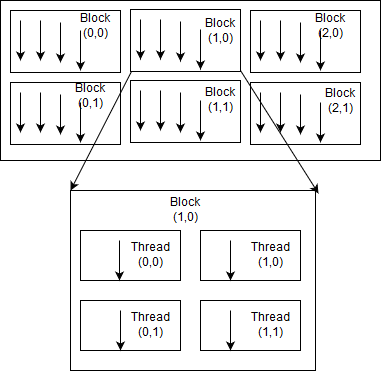
\includegraphics[width=10cm]{cudablock.png}
	\caption{2D grid with 6 thread blocks, each having 4 threads}
	\label{fig:cudablock}
\end{figure}
\squeezeup

\subsection{Pinned Memory}
Pinned memory can be accessed by the GPU and it can be read or written with a higher bandwidth when compared to pageable host memory. The memory allocation function malloc() allocates host memory on the heap, which is pageable by default. The GPU cannot access data directly from pageable host memory. Therefore, when a data is transferred from pageable host memory to device memory, the CUDA driver must first allocate a temporary page-locked, or pinned, host array, copy the host data to the pinned array, and then transfer the data from the pinned array to device memory. As shown in Fig. ~\ref{fig:pinned}, pinned memory is used as a temporary buffer when transferring data between the CPU and the GPU. Data transfer to the temporary buffer can be avoided by allocating data on pinned memory.

\begin{figure}[H]
	\centering
	\includegraphics[width=10cm]{pinned.png}
	\caption{Data transfer from the CPU to the GPU using pinned memory}
	\label{fig:pinned}
\end{figure}
\squeezeup

\section{CUDA Thread Execution Model}

The built-in variables blockDim and gridDim are used for specifying the number of threads in a block and the number of blocks in a grid \cite{bib5}. A thread block is identified by blockIdx and a thread in a thread block is identified by threadIdx. The variables blockIdx and threadIdx have member variables that represent the x, y and z components. For a one-dimensional kernel, threadIdx.x uniquely identifies a thread within a thread block and blockIdx.x uniquely identifies a block within a grid.

\subsection{Thread Synchronization}
Threads can be synchronized only across threads in a thread block by executing $syncthreads()$ function, but not across threads in a grid \cite{bib5}. There is no synchronization between thread blocks because thread blocks should execute independently on any SM without having to wait for other thread blocks. This allows CUDA applications to scale well with more SMs as thread blocks can be executed concurrently on multiple SMs.

\subsection{Thread Assignment}
During a kernel invocation, CUDA runtime assigns thread blocks to the SMs in the device \cite{bib5}. The programmer should ensure there are enough registers, shared memory and threads to execute the blocks. If resources are insufficient, the runtime will assign fewer thread blocks to the SM and the occupancy would decrease.

The total number of blocks that can be concurrently executed on an SM depends on the GPU model. Kepler architecture has a total of 13 SMs where each SM can execute up to 16 thread blocks \cite{bib5}. Thus, a Kepler GPU can run a total of 208 thread blocks concurrently. As each thread block in Kepler architecture can use up to 1024 threads, a total of 212,992 threads can concurrently run on one Kepler GPU.

An SM schedules threads in a group of 32 threads, which is referred to as a warp. In Kepler architecture, each SM has a quad-warp scheduler that selects four warps and dispatches two instructions from each warp every cycle.  As shown in Fig. ~\ref{fig:warpscheduler}, Kepler’s warp scheduler selects four warps, and two independent instructions per warp can be dispatched each cycle \cite{bib30}. 

In the Kepler architecture, up to 512 warps can be assigned to each SM. However, each clock cycle, only four warps out of the 512 warps are scheduled on an SM. Global memory accesses take over 400 cycles and can cause pipeline stalls. To hide the memory access latency, instructions from other warps are issued to an SM while the previous warp is waiting for its data.

\begin{figure}[H]
	\centering
	\includegraphics[width=10cm]{warpscheduler.png}
	\caption{A single warp scheduler unit}
	\label{fig:warpscheduler}
\end{figure}
\squeezeup

\subsection{Thread Divergence}
Thread divergence is caused due to branch statements such as if-then-else, switch and for \cite{bib5}. Divergence can only happen within a warp. When the branch condition is satisfied for some threads of a warp, the other threads of a warp that do not satisfy the condition are deactivated. For example, if eight threads of a warp evaluate an if condition to be true, then those eight threads will execute the conditional block and the remaining 24 threads will become idle. When the diverged flows merge, all 32 threads of a warp become activated.

The total execution time of a diverged warp is the accumulated execution time of all diverged flows. For example, PathA and PathB in Fig. ~\ref{fig:warpdivergence} are sequentially executed by a few threads within the same warp and hence, the total execution time is the accumulated execution time of PathA and PathB. One way to eliminate warp divergence is to have all threads in a block follow the same execution path. 

\begin{figure}[H]
	\centering
	\includegraphics[width=12cm]{warpdivergence.png}
	\caption{Thread divergence}
	\label{fig:warpdivergence}
\end{figure}
\squeezeup

\section{Signature Matching}
Signature matching inspects the packets payload to detect the presence of malicious network traffic by using various algorithms. The Rabin-Karp, the Wu-Manber and the Aho-Corasick algorithms were used to implement pattern matching.

\subsection{Rabin-Karp Algorithm}
In the Rabin-Karp algorithm \cite{bib19}, each thread computes hash code for the payload it operates on and compares it with hash code of well-known signature patterns. In the CPU-version Rabin-Karp algorithm, hash codes are computed for the neighboring values by using previously computed hash code and a new character. Thus, the run-time complexity of the algorithm is linear. However, the CPU-version algorithm cannot be used on the GPU because all threads execute in a parallel fashion. Hence, all threads compute hash-code up to the pattern length and compares it with hash code of the malicious patterns. Hash code computation and header inspection can be handled in parallel by using threads in different warps. In the Rabin-Karp algorithm, global memory accesses are highly coalesced. Therefore, the Rabin-Karp algorithm outperforms the naive algorithm.

The Rabin-Karp algorithm uses hashing. Considering an example in which the hash table size is 97 and the search pattern is 59372. Hash value is computed as 59372 \% 97, which is 8. Hash values of a set of numbers are shown in Table ~\ref{tab:hashvalue}.

\begin {table}[H]
\caption {Hash Value Calculation Example (Pattern = 59372)} \label{tab:hashvalue}
\begin{tabular}{|c|c|c|c|c|c|c|c|c|c|}
	\midrule
	idx 0 & idx 1 & idx 2 & idx 3 & idx 4 & idx 5 & idx 6 & idx 7 & idx 8 & Hash Value\\
	\midrule
	3 & 1 & 5 & 9 & 3 & 7 & 2 & 6 & 3 &\\
	\midrule
	3 & 1 & 5 & 9 & 3 & & & & & 31593\%97=68 \\
	\midrule
	& 1 & 5 & 9 & 3 & 7 & & & & 15937\%97=29\\
	\midrule
	&   & 5 & 9 & 3 & 7 & 2 & & & 59372\%97=8 \\
	\midrule
	&   &   & 9 & 3 & 7 & 2 & 6 & & 93726\%97=24 \\
	\midrule
	&   &   &   & 3 & 7 & 2 & 6 & 3 & 37263\%97=20 \\
	\midrule
\end{tabular}
\end {table}
\squeezeup

The modulo hash function can be calculated in linear time using Horner's method \cite{bib29} and is represented as,

$X_i mod Q = (T_i*R^{M-1} + T_{i+1}*R^{M-2} + …….+ T_{i+M-1}* R^0) mod Q,$ 
where R is the range, which equals 10 for decimal numbers, and 256 for ASCII numbers. For this example, assume that R, Q, and M as 10, 97 and 5, respectively. $X_i$ is the number at index i. Then, $X_i mod Q$ is calculated as $(3 * 10000 + 1 * 1000 + 5 * 100 + 9 *10 + 3*1) \% 97$, which is 68. The calculations are shown in Table ~\ref{tab:hashtext}.

\begin {table}[H]
\caption {Hash Value Calculation Example with Horner's Method} \label{tab:hashtext}
\resizebox{\columnwidth}{!}{
	\begin{tabular}{|c|c|c|c|c|c|c|}
		\midrule
		I &  0 & 1 & 2 & 3 & 4 &\\
		\midrule
		0 & 3 & 1 & 5 & 9 & 3 &\\
		\midrule
		1 & (3)\%97=3 & & & & & \\
		\midrule
		2 & 3 & 1 &  (3*10 + 1)\%97 = 31 & & &\\
		\midrule
		3 & 3 & 1 & 5 &  (31*10 + 5)\%97= 24 & &\\
		\midrule
		4 & 3 & 1 & 5 & 9 & (24*10 + 9)\%97 = 55 & \\
		\midrule
		5 & 3 & 1 & 5 & 9 & 3 & (55*10 + 3)\%97 = 68 \\
		\midrule
	\end{tabular}
}
\end {table}
\squeezeup

The resultant value after applying the hashing algorithm can match for two numbers.
For example, 59372 \% 97 = 95 and 59469 \% 97 = 95. Thus, the potentially matching patterns are compared against the text to see if there is a match. The time complexity of the algorithm is $O(NM)$, where N is the length of the text and M is the length of the pattern.

This algorithm can be optimized by calculating the next hash value by using the previous hash value. The next hash value $X_{i+1} mod Q$ can be computed efficiently by using the previous hash value $X_i mod Q$. 

We have, $X_i = T_i*R^{M-1} + T_{i+1} * R^{M-2} + …..+ T_{i+M-1} * R^0 $ and $X_{i+1} = T_{i+1}*R^{M-1} + T_{i+2} * R^{M-2} +…….+ T_{i+1+M-1}*R^0.$ Thus, $X_{i+1} =  (X_i - T_i*R^{M-1}) * R  + T_{i+M}.$ 


Suppose that, $X_i$ (current value) = 31593, $X_{i+1}$ (next value) = 15937, i = 0, $T_i$ = 3, $R^{M-1}$ = 10000, R = 10, M = 5, and $T_{i+M}$ = 7. When the above formula is applied, $X_{i+1} = (31593 - 3*10000)*10 + 7 = 15937.$ After obtaining the next hash value, $X_{i+1} mod Q$, it should be compared with the hash value of the pattern.

Thus, the time complexity of single pattern matching is $O(N)$. When a single pattern-matching algorithm is used for multi-signature matching, the same algorithm is applied to every signature. Hence, the time complexity for multi-pattern matching is $O(N*MaxM)$ where $MaxM$ is the maximum pattern length.

\subsection{Aho-Corasick Algorithm}
The Aho-Corasick algorithm \cite{bib18} is one of the fastest algorithms for multi-pattern matching. The complexity of this algorithm is linear to the sum of the number of patterns, the length of the input text, and the total number of matches in the text. The algorithm has two phases, preprocessing and search. In the preprocessing phase, the algorithm builds a FSM that looks like a trie using a finite set of patterns. In the search phase, the algorithm traverses the input text along this state machine to find the locations of the patterns in the text.

In the preprocessing phase, three arrays, goto, failure, and output, are constructed.
\begin{enumerate}
	\item Goto array is a two-dimensional array and stores the next state for the current state and the currently processed character.  
	
	\item Failure array holds all the states that should be reached for those characters, that do not contain the next state for the current state. For example, in Fig. ~\ref{fig:failure}, when a state is 0 and the characters at this state are not h and s (!(h,s)), the arrow points back to state 0 (for state 0, any other characters other than h and s, have value 0). It is represented as a one-dimensional array.
	
	\item Output array stores the indexes of the patterns that end at a particular state. It is represented as a vector of bit-sets. For a designated state, there can be more than 64 patterns that end at that state. Hence, the data type of the output array cannot be chosen as an int or long. 
\end{enumerate}
\vspace{\topsep}

The algorithm constructs a trie as shown in Fig. ~\ref{fig:trie} and fills goto and output arrays. The algorithm extends the trie into a finite state automaton in order to achieve linear time complexity.

\begin{figure}[H]
	\centering
	\includegraphics[width=12cm]{trie.png}
	\caption{Trie is constructed for the patterns = {he, she, hers, his}}
	\label{fig:trie}
\end{figure}
\squeezeup

The value for a state in a failure array can be computed by finding the longest suffix of a pattern which is the prefix of another pattern. For example, consider the pattern “hers” as shown in Fig. ~\ref{fig:failure}, the longest suffix is “s,” which is the prefix of “she.” Thus, there is a failure transition from "hers" to “s” of “she.” While constructing the trie, for all characters that do not have the next state at the root, an edge is added back to the root. 

\begin{figure}[H]
	\centering
	\includegraphics[width=8cm, height=6cm]{failure.png}
	\caption{Trie is extended to include the failure transitions}
	\label{fig:failure}
\end{figure}
\squeezeup

Suppose that the search phase text is "ushers" as shown in Table ~\ref{tab:search}. The algorithm moves from state 0 to state 1 since the first character is a "u." At state 1, the output array is checked. Since the output value at state 1 index is 0, there is no pattern match. Similarly, the FSM is traversed to reach the next state from the present state depending on the input character. When the output array is checked at state 3 and state 9, it would have the bit corresponding to the pattern set to 1.

\begin {table}[H]
\centering
\caption {FSM Transition Example (Pattern = "ushers")} \label{tab:search}
	\begin{tabular}{|c|c|c|}
	\midrule
	CHARACTER & STATE & MATCHES\\
	\midrule
	u & 0 & NONE\\
	\midrule
	s & state 1 &  NONE\\
	\midrule
	h & state 2 & NONE\\
	\midrule
	e & state 3 & {he,she}\\
	\midrule
	r & state 8 & NONE\\
	\midrule
	s & state 9 & {hers}\\
	\midrule
\end{tabular}
\end{table}
\squeezeup

\subsection{Wu-Manber Algorithm}
The Wu-Manber algorithm \cite{bib16} is based on the idea of the Boyer-Moore algorithm \cite{bib17} and the search starts from right and proceeds to left. According to the Boyer-Moore algorithm, while searching in the text from right to left, if the rightmost character in the text does not match any of the characters in the pattern, a block of characters up to the pattern length can be skipped while searching and the search pointer can be moved to the right by the pattern length. The intuition is that, the right most character is likely to be different when the pattern doesn't match and hence, multiple characters can be skipped while searching and thus, improve the performance.

The algorithm consists of two phases, preprocessing and search. In the preprocessing phase, the shift and prefix tables are constructed. The shift table gives the value that is needed to shift from the current position with respect to the suffix of the patterns. The prefix table is indexed by the hash values of prefixes of the patterns, and contains the corresponding patterns as the value. When multiple patterns have the same hash value, the shift table stores the value which requires the minimum shift and the prefix table stores all the patterns that map to the hash value using a linked list. When a set of characters at the current position matches a suffix of a pattern, the shift value will be zero. When the value of the shift is zero, the prefix is calculated by considering the characters from 'current position - minimum pattern length' array index up to the current position, which serves as a key to the prefix table. 

Consider a text “ANDYMEETMESOONATGOOGLE” and patterns “SOON,” “COME” and “GOOGLE.” The minimum length of the patterns is four. The shift table and prefix table are constructed using sub-arrays of length four as shown in Table ~\ref{tab:shiftwuman}.

\begin {table}[H]
\centering
\caption {Shift Table Generated after Preprocessing} \label{tab:shiftwuman}
\begin{tabular}{|c|c|c|c|c|c|c|c|c|c|}
\midrule
SO &    OO &    ON &    CO &    OM &    ME &    GO &    OO &    OG   &    * \\
\midrule
2 & 1 & 0 & 2 & 1 & 0 & 2 & 1 & 0  & 3\\
\midrule
\end{tabular}
\end{table}
\squeezeup

Prefix table points to a list of patterns whose first B(2) characters are hashed as the index as shown in Table ~\ref{tab:prefix}.

\begin{table}[H]
\centering
\caption {Prefix Table Generated after Preprocessing} \label{tab:prefix}
\begin{tabular}{|c|c|c|}
\midrule
Index: hash of the prefix & Value: list of patterns with common prefix \\
\midrule
SO & SOON  \\
\midrule
CO & COME  \\
\midrule
GO & GOOGLE  \\
\midrule
\end{tabular}
\end{table}
\squeezeup

In the search phase, initially the last four characters of the text are only examined because four is the minimum pattern length. Later, the last two characters of the four characters are used for the hash computation. The calculated hash value is used for indexing the shift table. The search pointer is shifted by the value of the shift at every search. When the shift value is 0, the hash value of the first two characters of the four characters is used as the index for the prefix table. The patterns in the prefix table are compared with the text. When the pattern size is longer than four, additional characters from the text are included to continue the search. Considering the example, as shown in Table ~\ref{tab:searchwuman}.

In step 1, the index for DY will map to a wild character, *, in the shift table  because there is no pattern that has DY as the suffix. Hence, a maximum shift is applied, which is three.
In step 3, the index for ME will map to ME in the shift table because the pattern COME has ME as the suffix. Since the shift is 0, the hash value for ET is calculated and the prefix table is checked. As ET does not index to any value in the prefix table, the algorithm continues. Similarly, in step 5, the prefix table is accessed and the pattern "SOON" is compared against the text, and the result is a pattern match. 

\begin {table}[H]
\centering
\caption {Multi-Pattern Search on "ANDYMEETMESOONATGOOGLE" Using Pre-processed Shift and Prefix Tables} \label{tab:searchwuman}
\begin{tabular}{|c|c|c|c|c|}
\midrule
STEP & INDEX & SHIFT & PREFIX CHECK & RESULT\\
\midrule
1 & 3 & 3 & &\\
\midrule
2 & 6 & 3 & &\\
\midrule
3 & 9 & 0 & Yes & NoMatch\\
\midrule
4 & 10 & 3 & &\\
\midrule
5 & 13 & 0 & Yes & Match(SOON)\\
\midrule
6 & 14 & 3 & &\\
\midrule
7 & 17 & 2 & &\\
\midrule
8 & 19 & 1 & &\\
\midrule
9 & 20 & 0 & Yes & Match(GOOGLE)\\
\midrule
\end{tabular}
\end{table}
\squeezeup



\section{Parallelism in CPU Programming with OpenMP}
When a sequential program is executed on the CPU, only one core is used. However, if OpenMP is used, all the cores can be utilized because threads are evenly distributed across the cores. OpenMP follows the Fork-Join model, where the main thread starts and creates a set of worker threads \cite{bib31}. The number of threads to be created can be decided dynamically or can be specified at compile time. The worker threads are active in a parallel region, and when they exit it, they join with the main thread.

All threads in an OMP region are assigned to a thread block. Each OMP thread maps to one physical core, but more than one thread can be mapped to a core. 
Omp\_get\_num\_threads() function returns the number of threads, which is greater than one in the parallel region, and is one outside it. Omp\_get\_max\_threads() returns the number of cores in the CPU. 

Fig. ~\ref{fig:openmp} shows an example for an OpenMP program implemented in C. The for loop is split into multiple chunks and each thread executes one chunk of the for loop. Even when the compiler does not support OpenMP, the program yields correct output, but without parallelism.

\begin{figure}[H]
\centering
\begin{lstlisting}
int numOfProcessors = omp_get_max_threads();
omp_set_num_threads(numOfProcessors);
#pragma omp parallel for
for(int i=0;i<4;i++) {
c[i] = a[i] + b[i];
}
\end{lstlisting}
\caption{Example for an OpenMP program in C}
\label{fig:openmp}
\end{figure}
\squeezeup